\documentclass[10pt,letterpaper,onecolumn,draftclsnofoot]{IEEEtran}
\usepackage[margin=0.75in]{geometry}
\usepackage{listings}
\usepackage{color}
\usepackage{longtable}
\usepackage{graphicx}
\usepackage{float}
\usepackage{tabu}
\definecolor{dkgreen}{rgb}{0,0.6,0}
\definecolor{gray}{rgb}{0.5,0.5,0.5}
\definecolor{mauve}{rgb}{0.58,0,0.82}

\graphicspath{{../images/}}

\lstset{frame=tb,
language=C,
columns=flexible,
numberstyle=\tiny\color{gray},
keywordstyle=\color{blue},
commentstyle=\color{dkgreen},
stringstyle=\color{mauve},
breaklines=true,
breakatwhitespace=true,
tabsize=4
}

\setlength{\parindent}{0cm}

\begin{document}
\begin{titlepage}
	\title{CS 461 - Fall 2016 - Technology Review}
	\author{Matthew Johnson}
	\date{\today}
	\maketitle
	\vspace{4cm}
	\begin{abstract}
		\noindent Abstract goes here
	\end{abstract}

\end{titlepage}
\tableofcontents
\clearpage

\section{Programming Languages}

At the highest level, a main component of our software defined network
implementation is the programming language it is written in. This is an
important decision to make early in our design, as it affects all choices that
follow.

\subsection{Options}

\subsubsection{Go}

Our first choice is the Go programming language. This is naturally the strongest
choice as the rest of the Ciao infrastructure is written in Go. It would require
a very strong argument to create a separate networking mode in another language.
While technically possible, it would require a great deal of work to make the
different pieces compatible with each other.

\subsubsection{C}

Other than interaction with the rest of the Ciao project, C is another natural
choice. C has been around for decades, and has the capability to do nearly every
computational and networking task. The libraries are extensive and available and
the language is fast.

\subsubsection{Python}

Python is a choice here simply because of its ease of use. Python is very
expressive and has nice libraries that abstract away the complicated details of
software defined networking. The main downfalls of Python, however, are its
reduced speed and space efficiency compared to Go and C. A result of writing a
cloud orchestrator in Python is exemplified in the extremely complicated and
slow Openstack project~\cite{uglyopenstack}.

\subsection{Goals for use in design}

As stated, the choice of programming language will affect all aspects of our
design for this project, from code structure to networking libraries and module
design. This choice will easily have the largest impact on our project.

\subsection{Criteria being evaluated}

Important criteria to consider is the availability of necessary libraries and of
the language and its dependencies itself, the inherent speed of the language to
be used, the security features the language offers, the concurrency
capabilities, and the overall ease of use.

\subsubsection{Availability}

The most available language in terms of libraries and the language itself
(regarding its standard libraries) is obviously C because of how ubiquitous it
is, how universally available it is, and how extensive its standard libraries
are~\cite{SOC}.

Close behind C in availability is Python. Python is nearly as available as C is
because of how popular it has become in the last ten years~\cite{PYPL}. Python
has many libraries that provide simple abstractions to networking
functionalities.

Of all these languages, Go is the least available as it is the youngest and
least popular of the three. Go is not normally available by default on most
operating systems and must be installed by the user. Go does, however, have
available libraries that make it very easy to implement networking, as is
evidenced by the extent to which they are used in the Ciao project
currently~\cite{ciao}.

The following figure demonstrates the popularity of C, Go, and Python in the
United States in the last ten years.

\begin{figure}[H]
	\begin{center}
		\makebox[\textwidth]{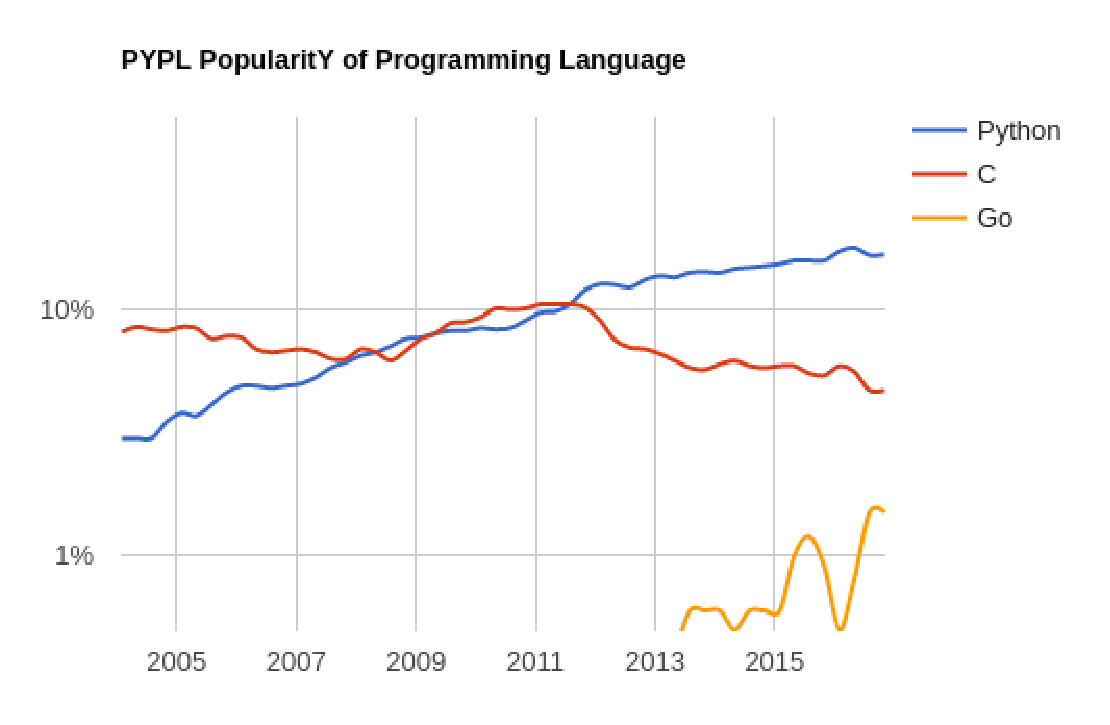
\includegraphics[width=10cm]{pythoncgo.eps}}
		\caption{Python, C, and Go popularity in the US~\cite{PYPL}}
	\end{center}
\end{figure}

\subsubsection{Speed and Space Efficiency}

One benefit of lower-level languages like Go and C is how they treat their
variables. Go and C treat variables differently than some languages such as
Python, which create overhead in order to track type information, and Java,
which converts small ints to Integer class instances when placing them in a
list. An example of this is in the representations of the same value in Go,
Python, and C~\cite{davecheney}:

\begin{lstlisting}
var gocon int32 = 2014              // Go:      4 bytes
uint32_t gocon = 2014;              // C:       4 bytes
gocon = 2014                        #  Python: 24 bytes
\end{lstlisting}

Go performs comparably to C with regard to speed, as well~\cite{benchmarks},
which is considerable since C is often the standard for fast programming
languages. Compared to Python, as would be expected, Go and C can perform up to
45 times faster depending on the workload~\cite{benchmarks}.

\subsubsection{Concurrency}

Concurrency is a key consideration for programming languages when implementing a
software defined network. All operations must happen quickly and in parallel and
must scale effortlessly. Therefore, it is necessary that all operations run in
their own individual threads.

C has an extensive and established framework for parallel computing by utilizing
pthreads. Mutexes can help the programmer protect against race conditions in
their code, but the responsibility is up to the programmer to make their
software thread-safe.

Python has similar tools as C, but the parallelization is handled by a global
interpreter lock (GIL). The GIL is a "mutex that prevents multiple native
threads from executing Python bytecodes at once." GIL is necessary in python
because the underlying C code that implements python is not thread-safe. The GIL
"prevents multithreaded CPython programs from taking full advantage of
multiprocessor systems in certain situations"~\cite{GIL}.

Go, on the other hand, combines the power of C and the ease of use and
lock-handling of Python. You can use goroutines (functions that are capable of
running concurrently with other functions) to create concurrency. Utilization of
goroutines and other builtin language functionalities make concurrency very easy
and lightweight in Go. An example from golang-book.com demonstrates how simple
and lightweight threads in Go can actually be~\cite{goroutines}:

\begin{lstlisting}
package main

import "fmt"

func f(n int) {
	for i := 0; i < 10; i++ {
		fmt.Println(n, ":", i)
	}
}

func main() {
	go f(0)
	var input string
	fmt.Scanln(&input)
}
\end{lstlisting}

\subsubsection{Ease of use}

Python is by far the easiest to learn, use, and read. It focuses on
"readability, coherence, and software quality" and is recognized by many to be
extremely easy to use~\cite{learningpython}.

C, being the oldest and lowest-level language of the three, is not a simple
language to work with. Many things that are normally abstracted away in other
languages are required to be programmed explicitly by the programmer. String
manipulation is especially difficult in C.

Go is easier to learn than C and makes many improvements in terms of ease of
use. It was even designed this way. Go was designed to make programming
efficient in large-scale software development across teams with varying levels
of experience and skill. It was designed with "built-in concurrency and garbage
collection" and includes "rigorous dependency management."~\cite{godesign}.
These features are important for the work required by this project.

Another important note is that the rest of Ciao is written in Go, and while
possible to create interfaces from C or Python for Go, it would be very
difficult. Another option would be to re-implement Ciao in another language,
which is so difficult and time consuming that it cannot even be considered as an
option. With this consideration, Go is the clear winner in terms of ease of use.

\subsection{Direct Comparison}

\begin{center}
	\begin{tabular}{| l | l | l | l | l | l |}
		\hline
		Language & Availability & Efficiency & Concurrency & Ease of use
		\\ \hline
		Go     & 3 & 1 & 1 & 1 \\ \hline
		C      & 1 & 2 & 2 & 3 \\ \hline
		Python & 2 & 3 & 3 & 2 \\ \hline
	\end{tabular}
\end{center}

\subsection{Selection}

Based on the criteria explored above, the Go programming language is the
language we are selecting to implement our solution in. The remainder of the
technical review will be based on the assumption that we will be implementing
our solution in Go.

\section{Networking Libraries}

\subsection{Options}

\subsubsection{}

\subsubsection{}

\subsubsection{}

\subsection{Goals for use in design}

\subsection{Criteria being evaluated}

\subsubsection{Availability}

\subsubsection{Speed}

\subsubsection{Security}

\subsubsection{Concurrency}

\subsection{Discussion}

\subsection{Selection}

\section{Functional Testing Frameworks}

There are several testing frameworks available for Go. These range from the
basic and simple 'testing' library to the more complicated and in-depth GoConvey
and Ginkgo frameworks. Depending on our choice here, we could either add too
much extraneous work getting a testing framework setup, or we could end up with
simple tests that do not meet our needs.

\subsection{Options}

\subsubsection{Standard 'testing' library}

The simplest and most lightweight option is the standard 'testing' library. This
can be expanded with the additional 'testify' library, which adds functionality
for mocking, assertions, HTTP protocol, and basic functions.

\subsubsection{GoConvey}

GoConvey is a testing framework that allows you to track your test status with a
generated web UI. The tests can run automatically every time you save a .go
file. GoConvey also generates an html test coverage report that allows you to
review where your tests are falling short.

\subsubsection{Ginkgo}

GinkGo is a testing framework that allows you to write specifications for your
tests. It is lighter-weight than GoConvey and works primarily from the command
line. GinkGo takes a black box approach to testing.

\subsection{Goals for use in design}

The goal of the testing framework is to continuously verify our solution.
Testing is important for any software, but it is particularly important in cloud
orchestration networking. Our solution must be robust, and that can only be
verified through rigorous testing.

\subsection{Criteria being evaluated}

The two important criteria when selecting a testing framework is the
capabilities of the framework itself and the complexity of the framework. On one
hand we want the tests to be powerful and support important features such as
mocking and assertion. On the other hand we do not want the test framework to be
so complicated that it is difficult to write tests.

\subsubsection{Capability}

The most important aspect of the testing framework is its ability to perform
mocking. This is essential in unit testing. All three of the test frameworks
allow the programmer to perform mocking.

Another important capability is assertion testing. Once again, all three support
assertion tests.

A third important capability is randomization in testing. This is the best way
to ensure corner cases are hit. This aspect, however, is provided by the Go
standard library and therefore does not factor into this analysis.

One area where GoConvey shines is in its ability to perform testing analysis and
output an easy-to-use web user interface. Ginkgo also provides some extra
functionality related to black box testing.

\subsubsection{Complexity}

Of the three frameworks, the testing package is by far the simplest. Since it
exists in the standard library, there is no overhead of installation or setup to
get started writing tests~\cite{testing}.

Ginkgo is slightly more complicated to setup, since it is necessary to install
and run a few Ginkgo-specific commands before ready to start writing tests. Once
everything is ready, you can write tests, but must use Ginkgo-specific keywords
and tests to utilize its full potential~\cite{ginkgo}.

The most complex framework is the GoConvey suite. This is no surprise,
considering how powerful it is. GoConvey requires the programmer to view the
test results in a browser, as well~\cite{goconvey}. This is difficult for our
purposes, since we will be doing much of our development on remote machines via
ssh, and will not have access to an X server to view the results.

\subsection{Direct Comparison}

\begin{center}
	\begin{tabular}{| l | l | l |}
		\hline
		Framework & Capability & Complexity
		\\ \hline
		testing  & 3 & 1  \\ \hline
		GinkGo   & 2 & 2  \\ \hline
		GoConvey & 1 & 3  \\ \hline
	\end{tabular}
\end{center}

\subsection{Selection}
Although the direct comparison reveals that all three are equally averaged to
second place overall, the decision here is weighted towards the lowest in
complexity. Our solution will be complex and difficult to implement, we do not
want to have to worry about learning how to use a complicate testing framework
on top of everything else. The standard 'testing' package will be used for
functional and unit testing of our solution.

% Cody
\section{Packet Level Protocols}
One of the main components of our system is deciding which protocol will be
used to move data from one node to the next. Ciao provides its own data
transfer protocol using SSNTP. Comparing how SSNTP works in general to other
data transfer formats will provide insight into which protocol should be used.

\subsection{Options}

\subsubsection{SSNTP}
Simple and Secure Node Transfer Protocol is Intel's solution for the transfer
of data inside of Ciao networks. It is based on Transport Layer Security (TLS),
the defacto standard for secure data transfer over the Internet. Part of what
sets Ciao apart from the competition is its simplicity, as well as concise
message format.\cite{ssntp}

\subsubsection{TLS}
Transport Layer Security, or TLS, is the contemporary standard for secure data
transfer across the Internet. It was built as an improvement upon the Secure
Socket Layer protocol. It has great appeal as it is widely utilized, modern,
and well studied.\cite{tls}

\subsubsection{SSL}
Secure Socket Layer, or SSL, was the first version of what eventually became
TLS following its third major revision. Originally utilized in Netscape, it
wasn't widely utilized until it's third major revision. Secure Socket Layer
encrypts at the application layer, allowing broad general use. While being
somewhat older than the other protocols on the list, it is well understood and
the security has been well proven.\cite{ssl}

\subsection{Goals for use in design}
The primary goal of the selected protocol is fast, stable, secure, and
scalable communication between compute nodes and the orchestration node in
Ciao. These are simple, but critical goals for the project.

\subsection{Criteria being evaluated}
The criteria for each protocol will be their security capabilities, protocol
overhead, and ease of use. While stability is a concern, each protocol has
shown stability through implementation in other applications many times over.
This will be less of a focus for evaluation purposes.

\subsubsection{Speed}
Speed is a major consideration when working with a software defined network.
Our final selection for a protocol needs to be fast. Any major delays in
communication due to encryption or protocol overhead is a concern. While each
implementation of the protocol will have its pros and cons, here the focus
will be on application overhead to keep the metric in measurable territory.

SSL has two major components, the protocol, and the handshake protocol. The
handshake protocol is important as it ensures the overall security and
authenticity of the communication between point A and point B.
~\cite{topdown-ssl}

%Diagram of SSL handshake here
\begin{figure}[H]
	\begin{center}
		\makebox[\textwidth]{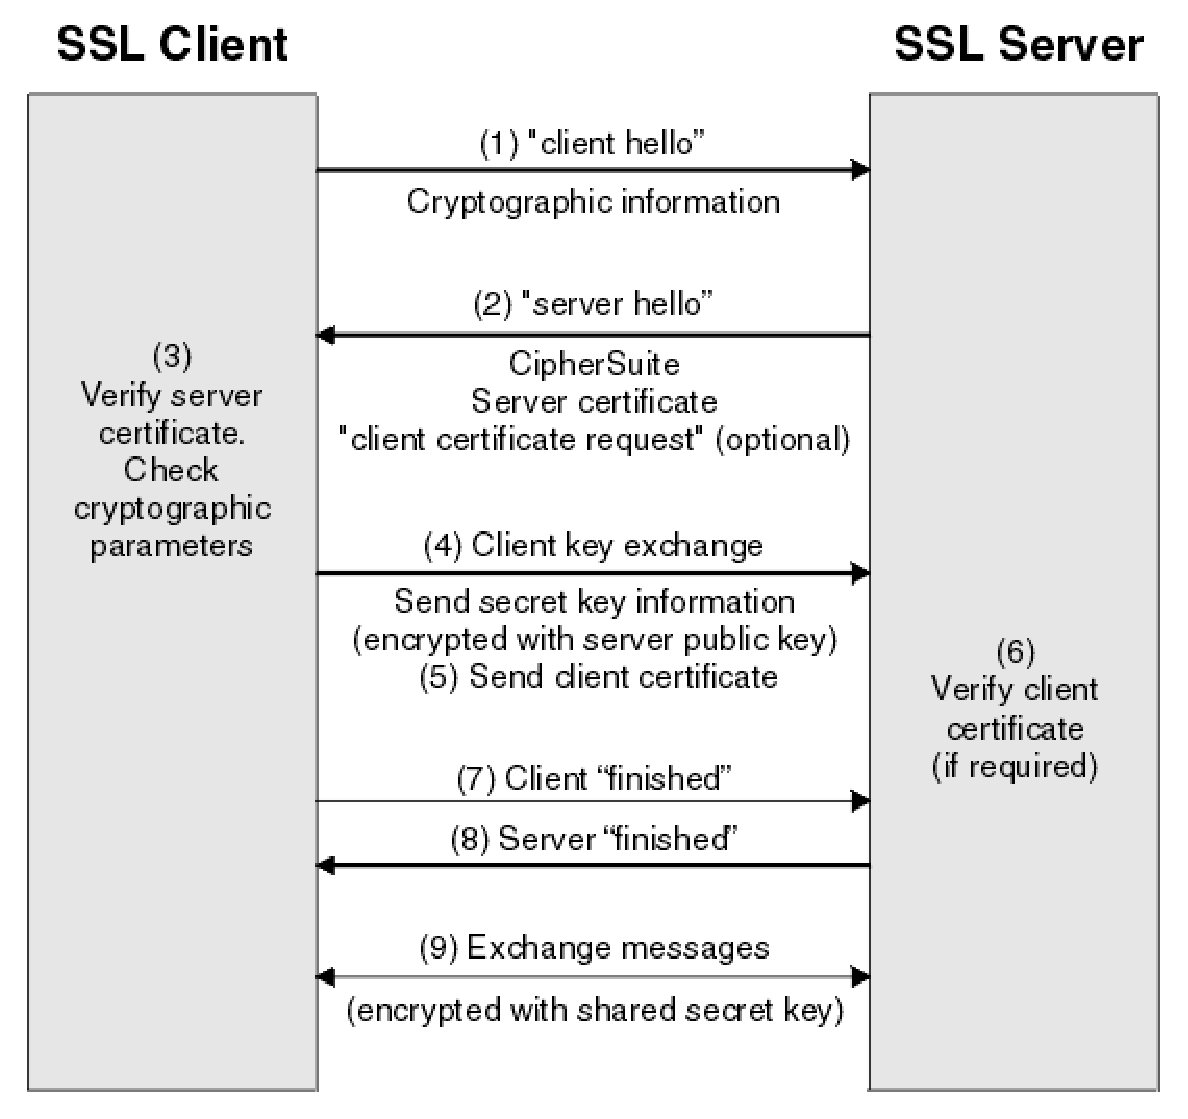
\includegraphics[scale=.35]{ssl-diag.eps}}
		\caption{Simple SSL and TLS Handshake\cite{ibm-diagram}}
	\end{center}
\end{figure}

The SSL/TLS handshakes are identical. As far as overhead the two protocols
are very similar. The primary difference between them is their security levels,
which will be discussed in the following section.

The SSNTP equivalent of a handshake is called a SSNTP Connection. There is a
fundamental difference that needs to be noted between SSNTP and the other two
options. The difference is that the computers running SSNTP client software
only have to do an authentication handshake, or SNTP Connection in this case,
once. Once the client knows which server it is talking to, all connections
no longer require a handshake step. This is a massive drop in needed overhead.
\cite{ssntp} Once the handshake is established, the client communicates with
the server in an asynchronous fashion as needed.

\subsubsection{Security}
Security is important in choosing a communication protocol. If it wasn't, we
could just use TCP, the protocol that all of these security protocols
encapsulate.

SSL is unfortunately at the bottom of the list as far as the
protocols listed here are concerned. Has a few vulnerabilities that have been
found in the decade or so. While some of these are less of an issue, one attack
in particular called POODLE has caused several major groups to call for SSL 3.0
to be deprecated.\cite{poodle} While calling into question consideration for
using this protocol on this system, it is still better than not having any
security or encryption at all.

TLS is much better on this front as it is continually being updated. The latest
release, version 1.2, uses AES, RC4, and a few other modern encryption ciphers.
\cite{tls} Which encryption cipher is used is negotiated between the host and
the client before communication begins.

SSNTP uses the TLS encryption protocols. On this front, it is equal to TLS.

\subsubsection{Accessibility}
All of the above protocols are well documented and easy to implement. In the
scope of the project, however, SSNTP would be easier to use because other
components of the system already use it. For that reason alone, it is simpler
to get working for the project.

\subsection{Direct Comparison}
Here is a side by side comparison of the protocols in the form of a table:

\begin{center}
	\begin{tabular}{| l | l | l | l |}
		\hline
		Protocol & Speed & Security & Accessibility \\ \hline
		SSNTP & 1 & 1 & 1 \\ \hline
		SSL & 2 & 3 & 2 \\ \hline
		TLS & 2 & 1 & 2 \\ \hline
	\end{tabular}
\end{center}

\subsection{Selection}
For our project, the technology for protocols will be SSNTP. It does what SSL
and TLS do equally security wise, but is much more light weight and is more
accessible in the context of the project.

%----------------------

\section{Network Virtualization}
Because Ciao works off of a virtual network, it's important to pick the right
tool for encapsulating packets to ensure they arrive at their destination. The
standard virtual network tools have proven to be limited in their ability to
scale. What the following tools do is allow for networks to scale to order of
magnatudes higher than a standard virtual network would. As for virtual networks
, virtual networks allow for virtual machines, or containers (docker, rkt) to be
visible to the virtual network switch. This is powerful as a VM or container
does not have a physical network card.

As we move to Open vSwitch, it gives us the option of using Network
Virtualization using Generic Routing Encapsulation (nvGRE) or Virtual Extensible
Local Area Network (VxLAN). Along with these two, a third option, Stateless
Transport Tunneling (STT), will be contrasted to see which option fits the
project needs best.

\subsection{Options}
\subsubsection{VxLAN}
VxLAN is a relatively new virtualization standard developed by a few major
players in the network industry. Cisco, VMware, Citrix, and Redhat all came
together to work on this standard to resolve the major problem of massive
virtual networks. VxLAN's primary advantage is that it has a massive address
space, about sixteen million, and that it's overall overhead increase is only
fifty bytes. \cite{vxlan} Speed will be a deciding factor in which interface
is chosen, so a fifty byte overhead is quite good.

\subsubsection{nvGRE}
NvGRE is another relatively new virtualization standard developed in tandum by
Microsoft, HP, Intel, HP, and Dell.\cite{nvgre-info} NvGRE sports a few of the
same features as VxLAN, the primary difference between the two being the header
field. They use different UDP port numbers and use a different bit to indicate
that encapsulation has occurred.\cite{nvgre} The primary difference between the
two is going to be overall performance in our network setup.

\subsubsection{STT}
Stateless Transport Tunneling is a protocol developed by VMware to handle the
same problem stated by the above protocols, but is primarily used to communicate
between virtual switches. It is quite different than the other protocols as it
carries much larger packets, up to sixty-four kilobytes, and it's overhead in
general is much larger. This could be a major problem when it comes to choosing
a protocol to use as overhead must be minimized.

\subsection{Goals for use in design}
The goal for these technologies is minimization of overhead while allowing for a
virtual network to be mapped and allow for thousands of VMs and containers to
become available easily. This problem of scalibility is a major one, and one
that has to be addressed when created large networks of computers hosting VMs or
virtual machines.

\subsection{Criteria being evaluated}
The primary attribute being evaluated here is performance or lack of overhead.
Performance and overhead go hand in hand, so they will be the primary metric of
evaluation for this project. In terms of speed, all of these protocols move at
the speed of hardware, so overhead makes sense for evaluation of the speed of
the protocol. Less overhead equals more packets moved per second.

\subsubsection{Overhead}
NvGRE and VxLAN share almost identical header formats, with the primary
difference in how they encapsulate their packets. NvGRE uses existing tunneling
functionality in a TCP packet to encapsulate the data. All that is different is
that is alters the twenty-four bits of data usually used for regular GRE to
identify itself. This quite useful as it allows a great deal of existing
hardware to support this "new" protocol. The primary downside here being that
loadbalancers and firewalls have to expand the the full packet, removing GRE, to
inspect the packet. This could be a major slowdown if the packet inspection is a
frequent activity.\cite{nvgre-vs-vxlan}

VxLAN on the otherhand, while adding an additional fifty bytes of overhead to
every packet, still requires the deencapsulation of every packet out of
the VxLAN format. The other downside here being reduced compatibility with
existing routing hardware. This is less of an issue for this project as all of
our routing devices will be implemented in software.\cite{nvgre-vs-vxlan}

STT has a significant disadvantage in the area of overhead when it comes to
general use. It's primary design purpose at VMware was to carry large amounts of
data from point A to point B. In our use case, it doesn't make much sense. Its
overall packet header size will be between sixty-two bytes to eighty bytes. This
is much larger than the other two. While this may not be a huge issue for VM to
VM traffic, it becomes an issue when it travels across physical networks.
\cite{stt}

\subsection{Direct Comparison}
\begin{center}
	\begin{tabular}{| l | l |}
		\hline
		Protocol & Overhead \\ \hline
		nvGRE & 1 \\ \hline
		VxLAN & 2 \\ \hline
		STT & 3 \\ \hline
	\end{tabular}
\end{center}

\subsection{Selection}
For the purposes of the project, we will work with nvGRE in order to provide the
lowest overhead. Live testing of nvGRE and VxLAN are part of the project. While
it is difficult to tell during the design phase which will be better in
production, on paper nvGRE seems to work better for our needs.

%----------------------

\section{GRE/Linux Bridges}

\subsection{Options}

\subsubsection{Linux Bridges}

\subsubsection{}

\subsubsection{}

\subsection{Goals for use in design}

\subsection{Criteria being evaluated}

\subsubsection{}

\subsubsection{}

\subsubsection{}

\subsubsection{}

\subsection{Direct Comparison}

\subsection{Selection}

\section{References}

\bibliographystyle{IEEEtran}
\bibliography{tech}

\end{document}
